\documentclass[10pt]{article}

\usepackage[
  letterpaper,
  top=0.78in,
  bottom=0.86in,
  left=1.02in,
  right=1.02in,
  headsep=17pt
]{geometry}
\usepackage[T1]{fontenc}
\usepackage{newpxtext}
\usepackage{newpxmath}
\usepackage[scale=0.94]{tgheros}
\usepackage{microtype}
\usepackage{setspace}
\usepackage{booktabs}
\usepackage{array}
\usepackage{tabularx}
\usepackage{enumitem}
\usepackage{graphicx}
\usepackage[hidelinks]{hyperref}
\usepackage[table]{xcolor}
\usepackage{tikz}
\usepackage{pgfplots}
\usepackage{placeins}
\usepackage[
  font={small,sf},
  labelfont={bf},
  labelsep=period,
  justification=raggedright,
  singlelinecheck=false
]{caption}
\usepackage{titlesec}
\usepackage{fancyhdr}

\pgfplotsset{compat=1.18}
\usetikzlibrary{arrows.meta, backgrounds, calc, positioning}

\definecolor{adlintink}{HTML}{111827}
\definecolor{adlintmuted}{HTML}{5B6472}
\definecolor{adlintline}{HTML}{D8DEE8}
\definecolor{adlintwash}{HTML}{F7F9FC}
\definecolor{adlintblue}{HTML}{2563EB}
\definecolor{adlintgreen}{HTML}{059669}
\definecolor{adlintorange}{HTML}{D97706}
\definecolor{adlintred}{HTML}{DC2626}
\definecolor{adlintviolet}{HTML}{7C3AED}

\AtBeginDocument{\color{adlintink}}
\setlength{\headheight}{14pt}
\setstretch{1.055}
\setlength{\emergencystretch}{2.5em}
\setlength{\parindent}{1.05em}
\setlength{\parskip}{0pt}
\setlength{\tabcolsep}{7pt}
\renewcommand{\arraystretch}{1.18}
\setlist{topsep=0.35em,itemsep=0.16em,parsep=0pt,leftmargin=1.45em}
\captionsetup{skip=0.46em}
\captionsetup[table]{position=top,justification=centering,singlelinecheck=true}

\hypersetup{
  pdftitle={AdLint Production Reliability and Live Model Evaluation},
  pdfauthor={AdLint Contributors},
  pdfsubject={Balanced real-case and local model evaluation for ad compliance review}
}

\titleformat{\section}
  {\sffamily\Large\bfseries\color{adlintink}}
  {\thesection}{0.62em}{}
\titleformat{\subsection}
  {\sffamily\large\bfseries\color{adlintink}}
  {\thesubsection}{0.56em}{}
\titlespacing*{\section}{0pt}{1.42em}{0.48em}
\titlespacing*{\subsection}{0pt}{0.98em}{0.32em}

\pagestyle{fancy}
\fancyhf{}
\fancyhead[L]{\sffamily\footnotesize\color{adlintmuted}AdLint reliability eval}
\fancyhead[R]{\sffamily\footnotesize\color{adlintmuted}May 2026}
\fancyfoot[C]{\sffamily\footnotesize\color{adlintmuted}\thepage}
\renewcommand{\headrulewidth}{0.3pt}
\renewcommand{\headrule}{\hbox to\headwidth{\color{adlintline}\leaders\hrule height \headrulewidth\hfill}}
\renewcommand{\footrulewidth}{0pt}
\fancypagestyle{plain}{%
  \fancyhf{}
  \fancyfoot[C]{\sffamily\footnotesize\color{adlintmuted}\thepage}
  \renewcommand{\headrulewidth}{0pt}
}

\newcolumntype{L}{>{\raggedright\arraybackslash}X}
\newcolumntype{P}[1]{>{\raggedright\arraybackslash}p{#1}}
\newcolumntype{R}[1]{>{\raggedleft\arraybackslash}p{#1}}
\newcommand{\dataset}{\texttt{real\_cases\_v1.jsonl}}
\newcommand{\modelname}{\texttt{gpt-oss-safeguard:20b}}
\newcommand{\metricnote}[1]{\textcolor{adlintmuted}{\sffamily\footnotesize #1}}
\newcommand{\eyebrow}[1]{%
  {\sffamily\scriptsize\bfseries\color{adlintmuted}\MakeUppercase{#1}}%
}
\newcommand{\stat}[2]{%
  \begin{tabular}{@{}c@{}}
    {\sffamily\bfseries\fontsize{18}{21}\selectfont\color{adlintink}#1}\\[-1pt]
    {\sffamily\scriptsize\color{adlintmuted}#2}
  \end{tabular}%
}

\newcommand{\summarybox}[2]{%
  \begin{center}
  \setlength{\fboxsep}{9pt}
  \fcolorbox{adlintline}{adlintwash}{%
    \begin{minipage}{0.92\linewidth}
      {\sffamily\bfseries\color{adlintink}#1}\par
      \vspace{0.24em}
      {\small #2}
    \end{minipage}%
  }
  \end{center}
}

\tikzset{
  flowbox/.style={
    rounded corners=2.25pt,
    line width=0.62pt,
    align=center,
    inner xsep=5pt,
    inner ysep=5pt,
    minimum width=2.62cm,
    minimum height=0.92cm,
    text width=2.38cm,
    font=\sffamily\footnotesize
  },
  rulebox/.style={flowbox, draw=adlintblue, fill=adlintblue!6},
  modelbox/.style={flowbox, draw=adlintorange, fill=adlintorange!8},
  reportbox/.style={flowbox, draw=adlintgreen, fill=adlintgreen!7},
  evalbox/.style={flowbox, draw=adlintviolet, fill=adlintviolet!7},
  flowarrow/.style={
    -{Latex[length=2.0mm,width=1.45mm]},
    line width=0.62pt,
    draw=adlintmuted,
    rounded corners=2pt
  },
  lanelabel/.style={
    font=\sffamily\scriptsize\bfseries,
    text=adlintmuted,
    anchor=west
  }
}

\pgfplotsset{
  adlint axis/.style={
    font=\sffamily\small,
    axis line style={adlintline},
    tick style={adlintline},
    tick label style={font=\sffamily\footnotesize,text=adlintmuted},
    label style={font=\sffamily\small,text=adlintmuted},
    title style={font=\sffamily\small\bfseries,text=adlintink},
    grid style={adlintline!55},
    major grid style={adlintline!55},
    axis x line*=bottom,
    axis y line*=left,
    clip=false,
    every axis plot/.append style={line width=0.72pt}
  },
  adlint bars/.style={
    adlint axis,
    xbar,
    width=0.82\linewidth,
    bar width=11pt,
    enlarge y limits=0.30,
    xmajorgrids=true,
    ymajorgrids=false,
    nodes near coords,
    point meta=x,
    nodes near coords style={
      font=\sffamily\footnotesize\bfseries,
      text=adlintink,
      anchor=west,
      xshift=2pt
    }
  }
}

\begin{document}
\thispagestyle{plain}
\vspace*{-0.32in}

\noindent\eyebrow{Technical report}\par
\vspace{0.28em}
\noindent{\sffamily\bfseries\fontsize{24}{28}\selectfont
AdLint Production Reliability and Live Model Evaluation\par}
\vspace{0.42em}
\noindent{\sffamily\large\color{adlintmuted}
Balanced public-source cases, rule diagnostics, and local-model quality evidence\par}
\vspace{0.72em}
\noindent{\sffamily\small\color{adlintmuted}AdLint Contributors \quad|\quad May 2026}

\vspace{1.0em}
\noindent\begin{tabularx}{\linewidth}{@{}XXXX@{}}
\stat{75}{real cases} &
\stat{25/25/25}{label balance} &
\stat{ok:75}{live model rows} &
\stat{0.493}{model-only accuracy}
\end{tabularx}

\summarybox{Bottom line}{%
The balanced real-case eval worked. It is reliable as production-reliability
diagnostic and regression coverage because it is sourced, deterministic,
schema-validated, and label-balanced. It is not a population-level proof of
platform approval accuracy because the cases are curated and paraphrased, not
random production traffic. The live model run shows that \modelname{} is
available but not ready to replace rules: model-only undercalled 38 rows, while
hybrid preserved rule accuracy with zero regressions.}

\section{Purpose}

AdLint is a local-first preflight system for ad copy, landing-page, privacy,
and brand-safety review. This report separates two questions that should not be
collapsed:

\begin{enumerate}
  \item \textbf{Production reliability diagnostics:} do the committed rules,
  labels, source metadata, and eval harness behave deterministically?
  \item \textbf{Live model value:} does the local model add precise review
  signal beyond the rule-only baseline?
\end{enumerate}

The current answer is clear. Rules remain the auditable decision backbone. The
local model can run on all real-case rows, but its current contribution is
mostly generic review narration rather than detailed YAML policy-id recall.

\section{Evaluation Design}

The eval suite now has three distinct layers. The synthetic rule benchmark is a
fast regression test. The public-source real-case set is a balanced diagnostic
for production reliability. The full local-model quality run is a manual or
scheduled evidence run, not a CI gate.

\begin{table}[!htbp]
\centering
\caption{Evaluation layers and intended use.}
\label{tab:eval-layers}
\small
\begin{tabularx}{\linewidth}{@{}P{0.25\linewidth}L P{0.22\linewidth}@{}}
\toprule
\textbf{Layer} & \textbf{Purpose} & \textbf{Gate type} \\
\midrule
\texttt{rule\_benchmark\_v1.jsonl} & Fast policy-engine regression coverage over 209 deterministic examples. & CI suitable \\
\dataset{} & Public-source diagnostic set with exact 25/25/25 decision balance and strict provenance metadata. & CI schema and rule-only diagnostic \\
\texttt{real-cases-model-quality} & Full live \modelname{} all-mode comparison with model-only, rule-only, and hybrid metrics. & Manual or scheduled quality run \\
\bottomrule
\end{tabularx}
\end{table}

\begin{figure}[!htbp]
\centering
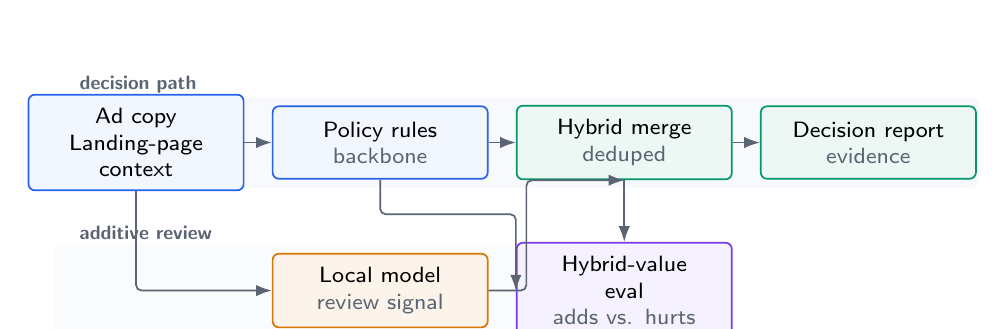
\begin{tikzpicture}[x=1cm,y=1cm]
\node[lanelabel] at (-0.84,0.74) {decision path};
\node[lanelabel] at (-0.84,-1.14) {additive review};

\node[rulebox] (input) at (0,0)
  {Ad copy\\Landing-page\\context};
\node[rulebox] (rules) at (3.1,0)
  {Policy rules\\\metricnote{backbone}};
\node[reportbox] (merge) at (6.2,0)
  {Hybrid merge\\\metricnote{deduped}};
\node[reportbox] (report) at (9.3,0)
  {Decision report\\\metricnote{evidence}};

\node[modelbox] (model) at (3.1,-1.88)
  {Local model\\\metricnote{review signal}};
\node[evalbox] (eval) at (6.2,-1.88)
  {Hybrid-value\\eval\\\metricnote{adds vs. hurts}};

\draw[flowarrow] (input) -- (rules);
\draw[flowarrow] (rules) -- (merge);
\draw[flowarrow] (merge) -- (report);
\draw[flowarrow] (input.south) |- ($(model.west)+(-0.12,0)$) -- (model.west);
\draw[flowarrow] (model.east) -- ++(0.48,0) |- (merge.south);
\draw[flowarrow] (rules.south) -- ++(0,-0.44) -| (eval.west);
\draw[flowarrow] (merge.south) -- (eval.north);

\begin{scope}[on background layer]
  \fill[adlintwash, rounded corners=3pt]
    (-1.04,-0.58) rectangle (10.70,0.58);
  \fill[adlintwash!72, rounded corners=3pt]
    (-1.04,-2.47) rectangle (7.58,-1.29);
\end{scope}
\end{tikzpicture}
\caption{Hybrid review architecture. Rules stay on the launch-decision path;
the local model is evaluated as additive review signal.}
\label{fig:architecture}
\end{figure}

\section{Balanced Real-case Set}

The real-case dataset has been rebuilt to 75 rows with exact decision balance.
Rows use paraphrased local inputs and public provenance metadata. Approved rows
must have empty \texttt{expected\_policy\_ids}; review and high-risk rows carry
the expected policy ids needed for deterministic diagnostics.

\begin{table}[!htbp]
\centering
\caption{Committed real-case dataset contract.}
\label{tab:real-case-contract}
\small
\begin{tabularx}{0.82\linewidth}{@{}L R{1.45cm}@{}}
\toprule
\textbf{Dataset property} & \textbf{Value} \\
\midrule
Total rows & 75 \\
Expected approved rows & 25 \\
Expected needs-review rows & 25 \\
Expected high-risk rows & 25 \\
Required source and provenance metadata & 7 fields \\
Live landing-page fetches committed & 0 \\
\bottomrule
\end{tabularx}
\end{table}

\begin{figure}[!htbp]
\centering
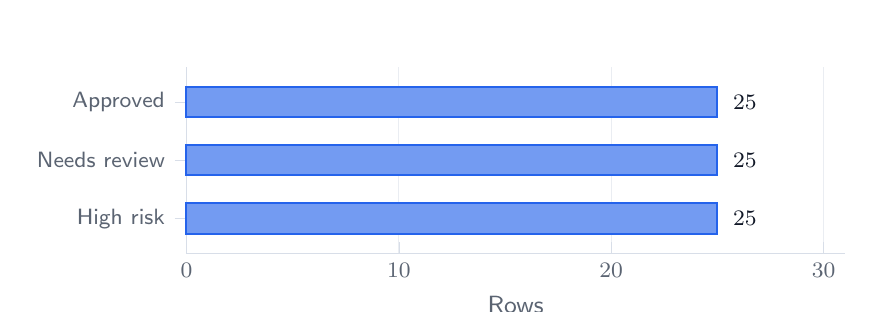
\begin{tikzpicture}
\begin{axis}[
  adlint bars,
  height=3.95cm,
  xmin=0,
  xmax=31,
  xlabel={Rows},
  symbolic y coords={High risk,Needs review,Approved},
  ytick=data,
  xtick={0,10,20,30},
  nodes near coords={\pgfmathprintnumber[fixed,precision=0]{\pgfplotspointmeta}}
]
\addplot[fill=adlintblue!64, draw=adlintblue] coordinates {
  (25,High risk)
  (25,Needs review)
  (25,Approved)
};
\end{axis}
\end{tikzpicture}
\caption{Decision-label balance in the public-source real-case dataset.}
\label{fig:real-case-balance}
\end{figure}

\section{Results}

\subsection{Rule and Hybrid Diagnostics}

Rule-only behavior is diagonal on the balanced real-case set. Hybrid preserves
that result when the model is available.

\begin{table}[!htbp]
\centering
\caption{Real-case all-mode result summary.}
\label{tab:mode-summary}
\small
\begin{tabular}{@{}lrrrlr@{}}
\toprule
\textbf{Mode} & \textbf{Rows} & \textbf{Skipped} & \textbf{Accuracy} & \textbf{Model status} & \textbf{Runtime} \\
\midrule
Rule-only & 75 & 0 & 1.000 & \texttt{disabled:75} & 0.993s \\
Model-only & 75 & 0 & 0.493 & \texttt{ok:75} & 599.513s \\
Hybrid & 75 & 0 & 1.000 & \texttt{ok:75} & 817.045s \\
\bottomrule
\end{tabular}
\end{table}

\begin{figure}[!htbp]
\centering
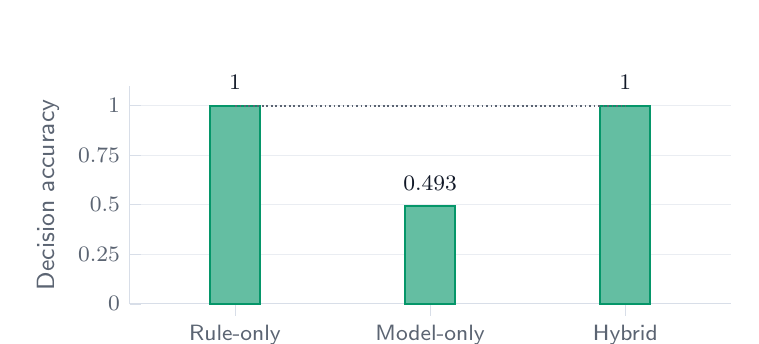
\begin{tikzpicture}
\begin{axis}[
  adlint axis,
  ybar,
  width=0.76\linewidth,
  height=4.35cm,
  ylabel={Decision accuracy},
  ymin=0,
  ymax=1.10,
  symbolic x coords={Rule-only,Model-only,Hybrid},
  xtick=data,
  ytick={0,0.25,0.50,0.75,1.00},
  ymajorgrids=true,
  xmajorgrids=false,
  bar width=18pt,
  enlarge x limits=0.27,
  nodes near coords,
  point meta=y,
  nodes near coords style={
    font=\sffamily\footnotesize\bfseries,
    text=adlintink,
    anchor=south,
    yshift=2pt
  },
  every node near coord/.append style={
    /pgf/number format/fixed,
    /pgf/number format/precision=3
  }
]
\addplot[fill=adlintgreen!62, draw=adlintgreen] coordinates {
  (Rule-only,1.000)
  (Model-only,0.493)
  (Hybrid,1.000)
};
\draw[densely dotted, draw=adlintmuted, line width=0.62pt]
  (axis cs:Rule-only,1.000) -- (axis cs:Hybrid,1.000);
\end{axis}
\end{tikzpicture}
\caption{Decision accuracy by mode on the balanced real-case dataset.}
\label{fig:mode-accuracy}
\end{figure}

\subsection{Model Quality}

The live model-quality run completed successfully: all 75 model-required rows
returned status \texttt{ok}. The model-only classifier still undercalled many
review and high-risk examples.

\begin{table}[!htbp]
\centering
\caption{Live \modelname{} quality findings.}
\label{tab:model-quality}
\small
\begin{tabularx}{0.86\linewidth}{@{}L R{1.55cm}@{}}
\toprule
\textbf{Metric} & \textbf{Value} \\
\midrule
Model OK rows & 75 \\
Model unavailable rows & 0 \\
Model-only decision accuracy & 0.493 \\
Model-only undercalls & 38 \\
Model-only overcalls & 0 \\
Hybrid decision regressions & 0 \\
Generic \texttt{model\_policy\_review} additions & 21 \\
Detailed expected YAML policy-id additions & 0 \\
Total all-mode runtime & 1417.551s \\
\bottomrule
\end{tabularx}
\end{table}

\begin{figure}[!htbp]
\centering
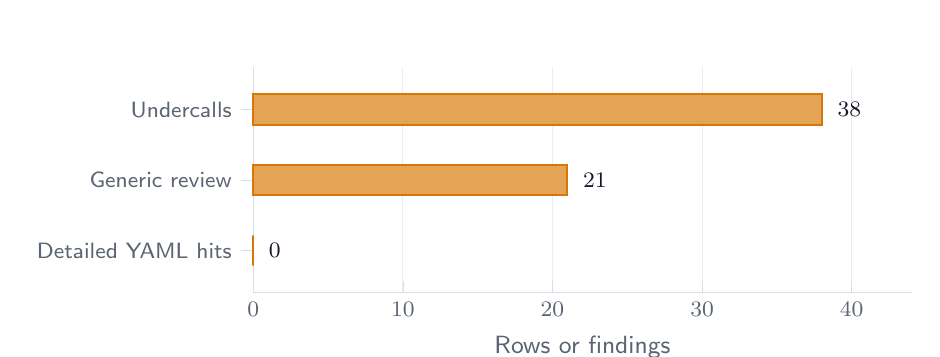
\begin{tikzpicture}
\begin{axis}[
  adlint bars,
  height=4.45cm,
  xmin=0,
  xmax=44,
  xlabel={Rows or findings},
  symbolic y coords={Detailed YAML hits,Generic review,Undercalls},
  ytick=data,
  xtick={0,10,20,30,40},
  nodes near coords={\pgfmathprintnumber[fixed,precision=0]{\pgfplotspointmeta}}
]
\addplot[fill=adlintorange!68, draw=adlintorange] coordinates {
  (0,Detailed YAML hits)
  (21,Generic review)
  (38,Undercalls)
};
\end{axis}
\end{tikzpicture}
\caption{The live model adds generic review notes, but not detailed expected
policy-id matches, and it undercalls a large share of risky rows.}
\label{fig:model-value}
\end{figure}

\subsection{Synthetic Rule Benchmark}

The synthetic benchmark remains useful as fast policy-as-code regression
coverage. It should not be read as external approval accuracy because examples
are authored for coverage rather than randomly sampled from production.

\begin{table}[!htbp]
\centering
\caption{Synthetic rule benchmark summary.}
\label{tab:rule-benchmark}
\small
\begin{tabularx}{0.78\linewidth}{@{}L R{1.6cm}@{}}
\toprule
\textbf{Metric} & \textbf{Value} \\
\midrule
Examples & 200 \\
Decision accuracy & 1.000 \\
Decision mismatches & 0 \\
Policy false-negative review notes & 0 \\
Policy false-positive review notes & 0 \\
Approved labels & 51 \\
Needs-review labels & 50 \\
High-risk labels & 99 \\
\bottomrule
\end{tabularx}
\end{table}

\section{Reliability Interpretation}

This is now a reliable eval for regression and diagnostic work:

\begin{itemize}
  \item Dataset shape is enforced by tests and \texttt{make real-cases-validate}.
  \item Each row has required source tier, rationale, provenance, access date,
  policy areas, copyright status, and outcome-source metadata.
  \item The committed real-case set has exact 25/25/25 decision balance.
  \item Rule-only and hybrid diagnostics are fast enough for local use and CI
  evidence.
  \item The live model-quality run proves model availability and exposes model
  value separately from fallback behavior.
\end{itemize}

It is not a reliability claim for all future ads or platform decisions. The
real-case rows are public-source and paraphrased, but still curated. The right
reading is: AdLint now has a strong regression harness and a credible
model-quality measurement loop; it does not yet have a statistically
representative production approval benchmark.

\section{Operating Gates}

\begin{table}[!htbp]
\centering
\caption{Recommended use of each eval gate.}
\label{tab:gates}
\small
\begin{tabularx}{\linewidth}{@{}P{0.29\linewidth}L P{0.20\linewidth}@{}}
\toprule
\textbf{Command} & \textbf{What it proves} & \textbf{Where it belongs} \\
\midrule
\texttt{make real-cases-validate} & Dataset metadata, source contract, duplicate ids, dates, enums, URL shape, and 25/25/25 balance. & CI gate \\
\texttt{make real-cases} & Rule-only diagnostic behavior over the committed real-case set. & CI diagnostic \\
\texttt{make real-cases-model-quality} & Full live local-model availability, model-only quality, hybrid deltas, undercalls, overcalls, and generic review noise. & Manual or scheduled \\
\bottomrule
\end{tabularx}
\end{table}

\section{Next Work}

The next highest-value work is not fine-tuning. It is better human-reviewed
model-value labels:

\begin{enumerate}
  \item Add cases where deterministic rules intentionally miss semantic or
  landing-page risk.
  \item Label whether generic \texttt{model\_policy\_review} notes are useful,
  noisy, or harmful.
  \item Track model-caused review burden separately from detailed policy false
  positives.
  \item Expand sourced real cases before using percentages as population-level
  reliability evidence.
  \item Revisit prompting or policy-id mapping before considering adapter
  training.
\end{enumerate}

\FloatBarrier

\end{document}
